\chapter{Feasibility of Full COSMO Weather Forecast Model on an FPGA Cluster}
Since we are unaware of the existance any usage of re-programmable hardware in large-scale simulations in practice at the time of writing, from the first day on we have been pursuing the legitimate question of feasibility. This section is dedicated to an early-on general resource usage estimation for COSMO and check if these constraints are satisfied by the, at the time of writing, state of the art FPGA, the Intel Stratix 10 FPGA. Since the complexity arises from the high number of abstraction layers imposed it is impractical to reason about the actual feasibility manually. That's why we started with the implementations and did the first feasibility study as soon as we progressed far enough with the StencilFlow framework to get substantial work done automatically. The following figure gives you an idea of the complexity and size of the COSMO dynamical core model.  
\begin{figure}[h]
	\centering
	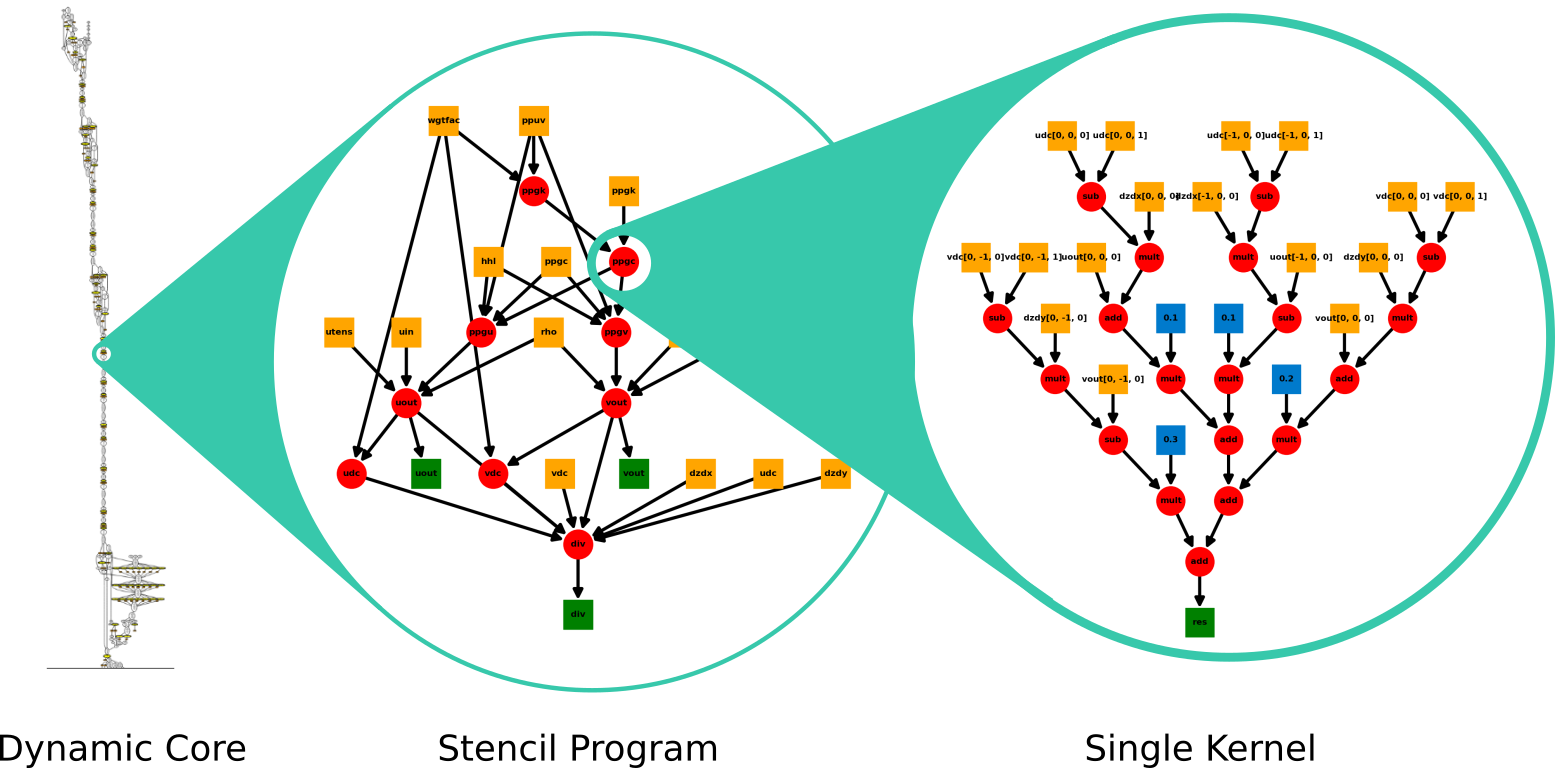
\includegraphics[height=16em]{drawings/dycore-estimate-complexity.png}
	\caption{The levels of abstraction: From the Dynamical Core to Stencil Programs and Kernels.}
	\label{fig:dycore-estimate-complexity2}
\end{figure}

\section{Estimation}

\paragraph{Assumptions}
Before we start with the derivation we want to summarize all the assumptions we made and justify their validity.

\subparagraph{Data Type}
According to discussions with experts from MeteoSwiss, most of the modeled equations converge by using floating point data types of 32 or 64 bit precision. Therefore we will assume that 32bit floating point precision (IEEE 754) is reasonable. The StencilFlow framework incorporates the functionality to choose a per-kernel data type, which would allow to choose the necessary precision on a per-equation basis. 

\subparagraph{Grid Size}
The current highest resolution, in-production variant has about 1158x774 horizontal and 80 vertical grid points (COSMO-1, COSMO-E: \\* 582x390x60, COSMO-7: 393x338x60) \cite{label51}. Together with experts from MeteoSwiss, we decided that grid sizes of 1024x1024x64, which is in the order of their current highest-resolution (1.1km) variant, would be a good choice.



\subparagraph{Iteration Space Order}
The dimension of the finite grid is not equally spaced in all three dimensions. The delay and internal buffer usage greatly depends on the order of iteration direction over the grid. Since there are no cycles in the data flow we assume that we can iterate over whichever direction is optimal. This can be achieved technically by either stream the transposed input data arrays to the FPGA or do it on the fly in a preprocessor transpose kernel. This modification saves us factor $\frac{1024}{64} = 16$ of buffer space.
\begin{minted}{python}
for (i = 0; i < X; i++)
  for(j = 0; j < Y; j++)
    for(k = 0; k < Z; k++)
      out[i,j,k] = f(S(in[i,j,k]))
\end{minted}
\begin{minted}{python}
for (i = 0; i < X; i++)
  for(j = 0; j < Y; j++)
    for(k = 0; k < Z; k++)
      out[i,k,j] = f(S(in[i,k,j]))
\end{minted}
\textit{Change the iteration direction order from X,Y,Z to X,Z,Y.}

\begin{figure}%
	\centering
	\subfloat{{
			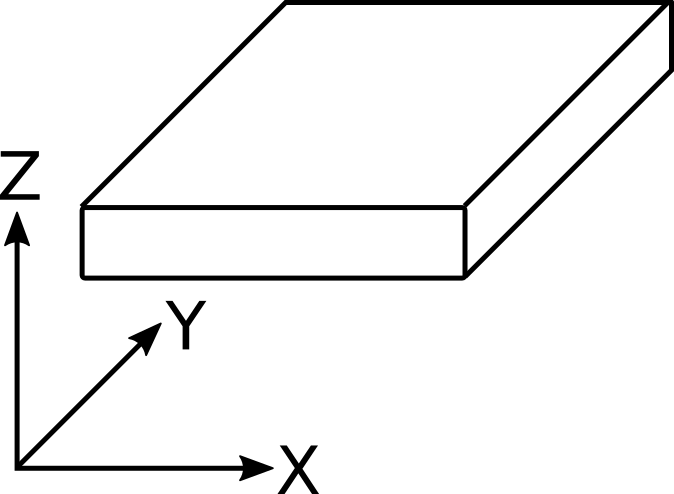
\includegraphics[width=.4\linewidth]{drawings/optimizer-iteration-xyz.png}
			 }}%
	\qquad
	\subfloat{{
			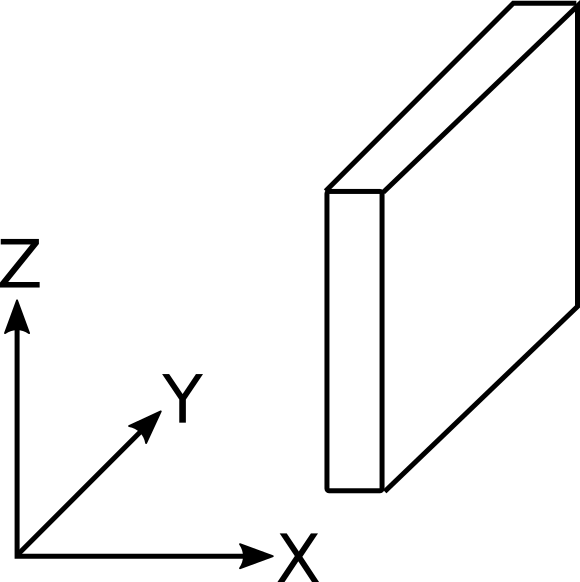
\includegraphics[width=.4\linewidth]{drawings/optimizer-iteration-xzy.png}
			 }}%
	\caption{Transposition of the input array to optimize buffer size.}
	\label{fig:optimizer-iteration-xyz-optimizer-iteration-xzy}
\end{figure}


\subparagraph{Dynamical Core}
To model the size, shape, critical path and delay buffer dependencies of the dynamical core of the weather forecast model, we used the high-level representation of the dependency graph (Runge Kutta time integration scheme). These values have been derived manually (total number of kernel programs) and partially automatically (critical path length, delay buffer size) by modeling the stencil programs as very simplistic stencils in the shape of the dependency graph. This lead to the following metrics, which we can later use with the average stencil program values to extrapolate to the full size.
\begin{itemize}
	\item Critical path length (in kernel programs): 252
	\item Total number of kernel programs: 131
	\item Delay buffer: 184 * buffer size of an average stencil program
\end{itemize}

\begin{figure}[h]
	\centering
	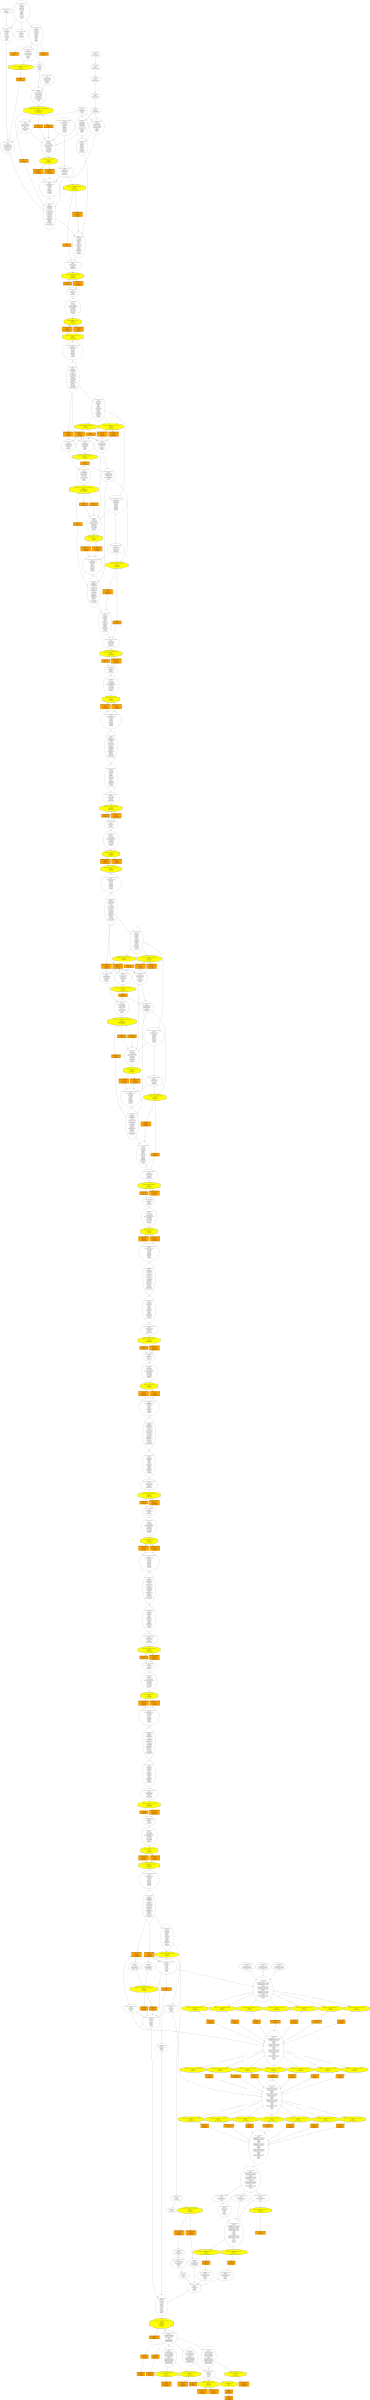
\includegraphics[height=36em]{drawings/dycore-overview.png}
	\caption{Overview over the stencil program of the whole dynamical core of COSMO. \textit{MeteoSwiss}}
	\label{fig:dycore-overview}
\end{figure}


\subparagraph{Average and Total Critical Path Length}  
The critical path length is the longest path from any input to the final output latency-wise.
\begin{itemize}
	\item fastwaves: [3, 1, 54]
	\item diffusion: [3, 0, 24]
	\item advection: [7, 4, 26]
	\item mean: $mean([[3, 1, 54]], [3, 0, 24], [7, 4, 26]) =$\\
	$ [\lceil\frac{3 + 3 + 7}{3}\rceil, \lceil\frac{1 + 0 + 4}{3}\rceil, \lceil\frac{54 + 24 + 26}{3}\rceil] = [5, 2, 35]$
	\item total critical path length = dycore critical path length * mean path length $ = 252 * [5, 2, 35] = [1260, 504, 8820]$
\end{itemize}


\subparagraph{Average and Total Buffer Size}
In order to estimate the buffer space of the whole model, we manually converted three common stencil programs of COSMO, namely fastwaves, advection and diffusion, to the StencilFlow input format and let the tool analyze their buffer usage. We use the average of them for extrapolation.

\begin{itemize}
	\item fastwaves: 
	\begin{itemize}
		\item internal buffer: [8, 7, 6]
		\item delay buffer: [32, -12, 289]
		\item combined: [40, -5, 295]
	\end{itemize}
	\item diffusion: 
	\begin{itemize}
		\item internal buffer: [16, 13, 0]
		\item delay buffer: [20, 8, 192]
		\item combined: [36, 21, 192]
	\end{itemize}
	\item advection: 
	\begin{itemize}
		\item internal buffer: [8, 8, 0]
		\item delay buffer: [10, 2, 57]
		\item combined: [18, 10, 57]
	\end{itemize}
	\item mean delay buffer: $mean([32, -12, 289], [20, 8, 192], [10, 2, 57]) = $\\
	$ [\lceil\frac{32 + 20 + 10}{3}\rceil, \lceil\frac{-12 + 8 + 2}{3}\rceil, \lceil\frac{289 + 192 + 57}{3}\rceil] =	[21, 0, 180]$

	\item mean combined buffer: $mean([40, -5, 295], [36, 21, 192], [18, 10, 57]) = [\lceil\frac{40+36+18}{3}\rceil, \lceil\frac{-5 + 21 + 10}{3}\rceil, \lceil\frac{295 + 192 + 57}{3}\rceil] = [32, 9, 182]$
	
	\item total delay buffer = dycore delay buffer estimate (unit: size of average stencil program buffer size) * average combined buffer size = $184 * [32, 9, 182] = [5888, 1656, 33488]$
\end{itemize}


\subparagraph{Average i-th Largest Buffer}
For the sake of simplicity, we use the natural heuristic optimization strategy for the manual estimate. First, we assume all buffers to be allocated in the fast memory of the FPGA, and we swap out the largest buffer of each stencil program to slow memory till we reach the memory bandwidth bottleneck. In order to achieve this, we manually looked at our three stencils and calculated their buffer sizes in Megabytes for the largest 10 buffers and computed the mean. The values are as follow:
$[\approx 3.7MB, \approx 0.8MB, \approx 0.6MB, \approx 0.4MB, \approx 0.4MB, \approx 0.4MB, \approx 0.3MB, \approx 0.2MB, \approx 0.2MB]$. This gives us the following fast memory savings per stencil program, if we stream the data to slow memory (swap out).
\begin{itemize}
	\item 1 buffer evicted:  $\approx 3.7MB$
	\item 2 buffers evicted:  $\approx 4.5MB$
	\item 3 buffers evicted:  $\approx 5.1MB$
	\item 4 buffers evicted:  $\approx 5.5MB$
	\item 5 buffers evicted:  $\approx 5.9MB$
	\item 6 buffers evicted:  $\approx 6.3MB$
	\item 7 buffers evicted:  $\approx 6.6MB$
	\item 8 buffers evicted:  $\approx 6.8MB$
	\item 9 buffers evicted:  $\approx 7.1MB$
	\item 10 buffers evicted:  $\approx 7.3MB$
\end{itemize}
\textit{Remark: Depending on the actual hardwares bandwidth capacity, we might go a lot higher than swapping out 10 buffers evicted per stencil program, but it is infeasible to go ahead manually, since the complexity of extraction increases.}


\subparagraph{Clock Frequency}
In contrast to modern CPU and GPU architectures, the FPGA frequency is flexible per design (in a range of tens or hundreds of Megahertz), but fixed after the synthesis has been finished. Expertise from previous projects have shown that 200-300Mhz is a reasonable assumption that should be achievable with todays FPGA devices \cite{label59}.

\subparagraph{Pipeline Theory}
We assume to deal with a ideal pipeline, which means we will have a saturation phase a full utilization phase and a draining phase, where we are able to produce one output per clock cycle in the latter two phases.


\paragraph{Derivation}
We will split the derivation into two subproblems. First we want to find out how many cycles it takes from the feed of the first data element till the last result exits the pipeline. This gives us an upper bound on the communication volume available. In a second step, we want to find out how much communication volume is required to move all data elements to respectively from the FPGA.

\subparagraph{Latency}
The critical path length of the dynamical core is 252 stencil programs. Since every stencil program itself has an average latency of [5, 2, 35], we end up with a total latency of $252 * [5, 2, 35] = [1260, 504, 8820]$ \\
The grid is 1024x1024x64 (longitude x latitude x altitude) in size. We would like to optimize the total buffer usage by reordering the dimensions to [64, 1024, 1024] = [X,Y,Z]. This leads to the absolute latency value (in cycles) of: $(8820*1 + 504*X + 1260*X*Y) = (8820 + 504*64 + 1260*64*1024) = 82616436$ cycles. \\
Under the assumption that we can produce one result every cycle after the pipeline is saturated, we et the following latency:
\begin{itemize}
	\item total run time (cycles): $latency + X*Y*Z = 82616436 + 64*1024*1024 = 149725300$ cycles
	\item total run time (seconds): $\frac{149725300 cycles}{200MHz} = 0.7486265$ seconds
\end{itemize}


\subparagraph{Communication Volume}
We will derive the total communication volume for the scenario of swapping out all delay buffers to slow memory since they are a lot larger in the analyzed designs (\textit{Remark: The actual size might still be smaller, since almost every field access imposes internal buffer, but only very few do impose delay buffers.}) compared to the internal buffers. Beside that, we move the 10 largest buffers of each stencil program from fast memory to slow memory while residing the remaining buffer allocations in fast on-chip memory. \\
From the dycore delay buffer estimate (184) and the average stencil program buffer size, we derive the total amount of delay buffer: $184 * [32, 9, 182] = [5888, 1656, 33488]$ in dimensional form. Using the transposed input dimensions and the float32 assumption, we get: $184 * 4bytes * [32, 9, 182] = 4bytes * 184 * (182 + 64*9 + 32*64*1024) = 184 * 8391640bytes \approx 184* 8.39MB = 1544061760bytes \approx 1544MB$. Since we have to move that data from the fast memory to the slow memory and back, we have to account twice for the communication volume: $2 * 1544MB = 3088MB$ \\
Buffering the 10 largest channels in slow memory gives us an approximate saving of 7.3MB per stencil program, which is half of the total communication volume (we have to bring the data elements out and in again), which leads to: $2 * 131 * 7.3MB = 1912.6MB$ \\
This gives us a total communication volume: $3088MB + 1912.6MB = 5000.6MB$ \\
The next step will be now to look at the specifications of a state of the art FPGA to find out if these numbers are feasible.


\subparagraph{Fast and Slow Memory}
We finally need to derive the fast and slow memory requirements imposed by the above optimization strategy. \\
The slow memory size is equal to the combination of all the delay buffers and the 10 largest internal buffers: $(131 + 184) * 8.39MB = 2642.85MB$.\\
The fast memory contains all the internal buffers that are smaller then the 10 largest ones: $(8.39MB - 7.3MB) * 131 = 142.79MB$

\begin{center}
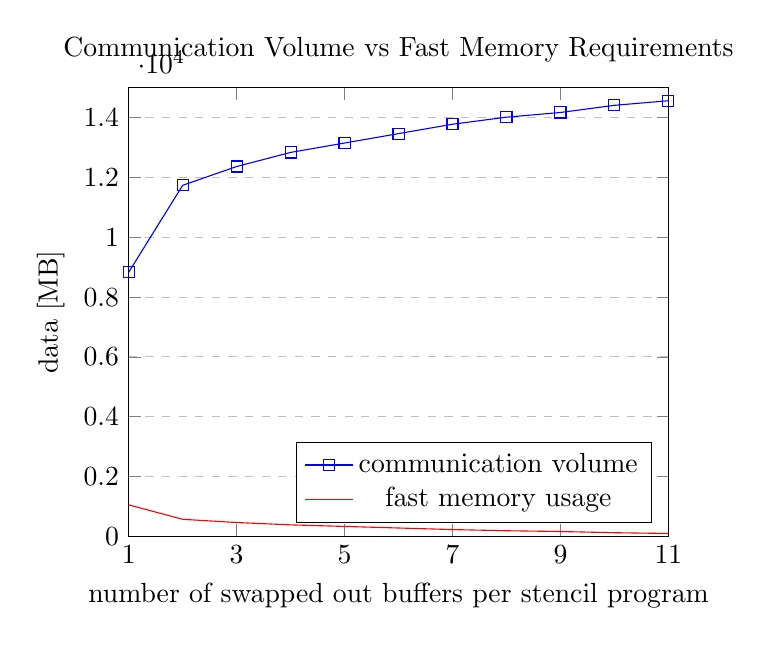
\begin{tikzpicture}
\begin{axis}[
title={Communication Volume vs Fast Memory Requirements},
xlabel={number of swapped out buffers per stencil program},
ylabel={data [MB]},
xmin=1, xmax=11,
ymin=1, ymax=15000,
xtick={1,3,5,7,9,11},
ytick={0,2000,4000,6000,8000,10000,12000,14000},
legend pos=south east,
ymajorgrids=true,
grid style=dashed,
]
\addplot[
color=blue,
mark=square,
]
coordinates {
	(1,8832)(2,11740.2)(3,12369)(4,12840.6)(5,13155)(6,13469.4)(7,13783.8)(8,14019.6)(9,14176.8)(10,14416)(11, 14569.8)
};


\addplot[
color=red,
mark=circle,
]
coordinates {
	(1,1048)(2,566)(3,458.5)(4,379.9)(5,327.5)(6,275.1)(7,222.7)(8,183.4)(9,157.2)(10,117.9)(11,91.7)
};
\legend{communication volume, fast memory usage}
\end{axis}
\end{tikzpicture}
\end{center}


\section{Case Study: Intel Stratix 10 FPGA}
This section is dedicated to the important technical aspects necessary to check if the above constraints can be fulfilled by a state of the art FPGA. We have chosen the Intel Stratix 10 FGPA since it is one of the most advanced re-programmable hardware on the market at the time of writing and we do have lots of such devices available at CSCS and the University of Paderborn. Nevertheless, this walk through is representative for other devices too. \\


\subparagraph{Parameters}
The key metrics for our optimization objective are:
\begin{itemize}
	\item fast on-chip memory: 25MB
	\item slow dram memory: 64GB
	\item memory bandwidth between slow and fast memory: 86.4GB/s
	\item clock frequency: theory: up to 1GHz, observed in synthesized stencil programs: 250-350Mhz
\end{itemize}
The reason we rely only on these very few parameters for estimating the feasibility is that we are following the basic assumption that our stencil programs are heavily memory bound. In addition to that, the DSP blocks on these devices offer a huge amount of parallel available operation processing power that we do not think this will constrain us. The Stratix 10 can deliver up to $10^12$ floating point operations per second.


\subparagraph{Bandwidth}
A single run of the program takes 0.749 seconds, which allows us at a memory bandwidth rate of 86.4GB/s to transfer $\frac{86.4GB}{s} * 0.749s = 64.7136GB$ of data. Since we only need 5000.6MB of communication volume, we are within the constraints, even with a high level of communication overhead.


\subparagraph{Slow Memory}
The derivation has shown that we need 2642.85MB of slow memory to allocate all the swapped out buffers. Since we have 64GB available, we are perfectly within the constraints.


\subparagraph{Fast Memory}
The derivation has shown that we need 142.79MB of fast memory if we use the naive optimization scheme from above. This would mean that we need $\lceil\frac{142.79MB}{25MB}\rceil = 6$ FPGA devices to fit the whole design. \textit{Remark: The high excess of memory bandwidth and slow memory would suggest to further swap out buffers, which would potentially make the design fit on fewer or even a single FPGA device. This will be part of the automatic optimization framework to find a good balance between these constraints.}


\section{Conclusion}
We could show that even with a naive optimization strategy, we should be able to fit the whole dynamical core of the COSMO weather prediction model onto six Intel Stratix 10 FPGA devices. Further optimization might significantly reduce this number, since there is lot of headroom for the bandwidth and slow memory utilization. In addition to that, multi FPGA designs are not only possible in theory, but are rather something we consider to achieve in the future either for fitting larger problems or to accelerate the current design. Especially the shape with large depth and small width of the COSMO weather models looks promising for a simple splitting of design without imposing a lot of data streams between the devices. The collaboration with the University of Paderborn and their configuration of 32 Stratix 10 FPGAs connected through 40Gbps direct optical fiber links will help us to achieve our goal \cite{label60}.
\begin{figure}[h]
	\centering
	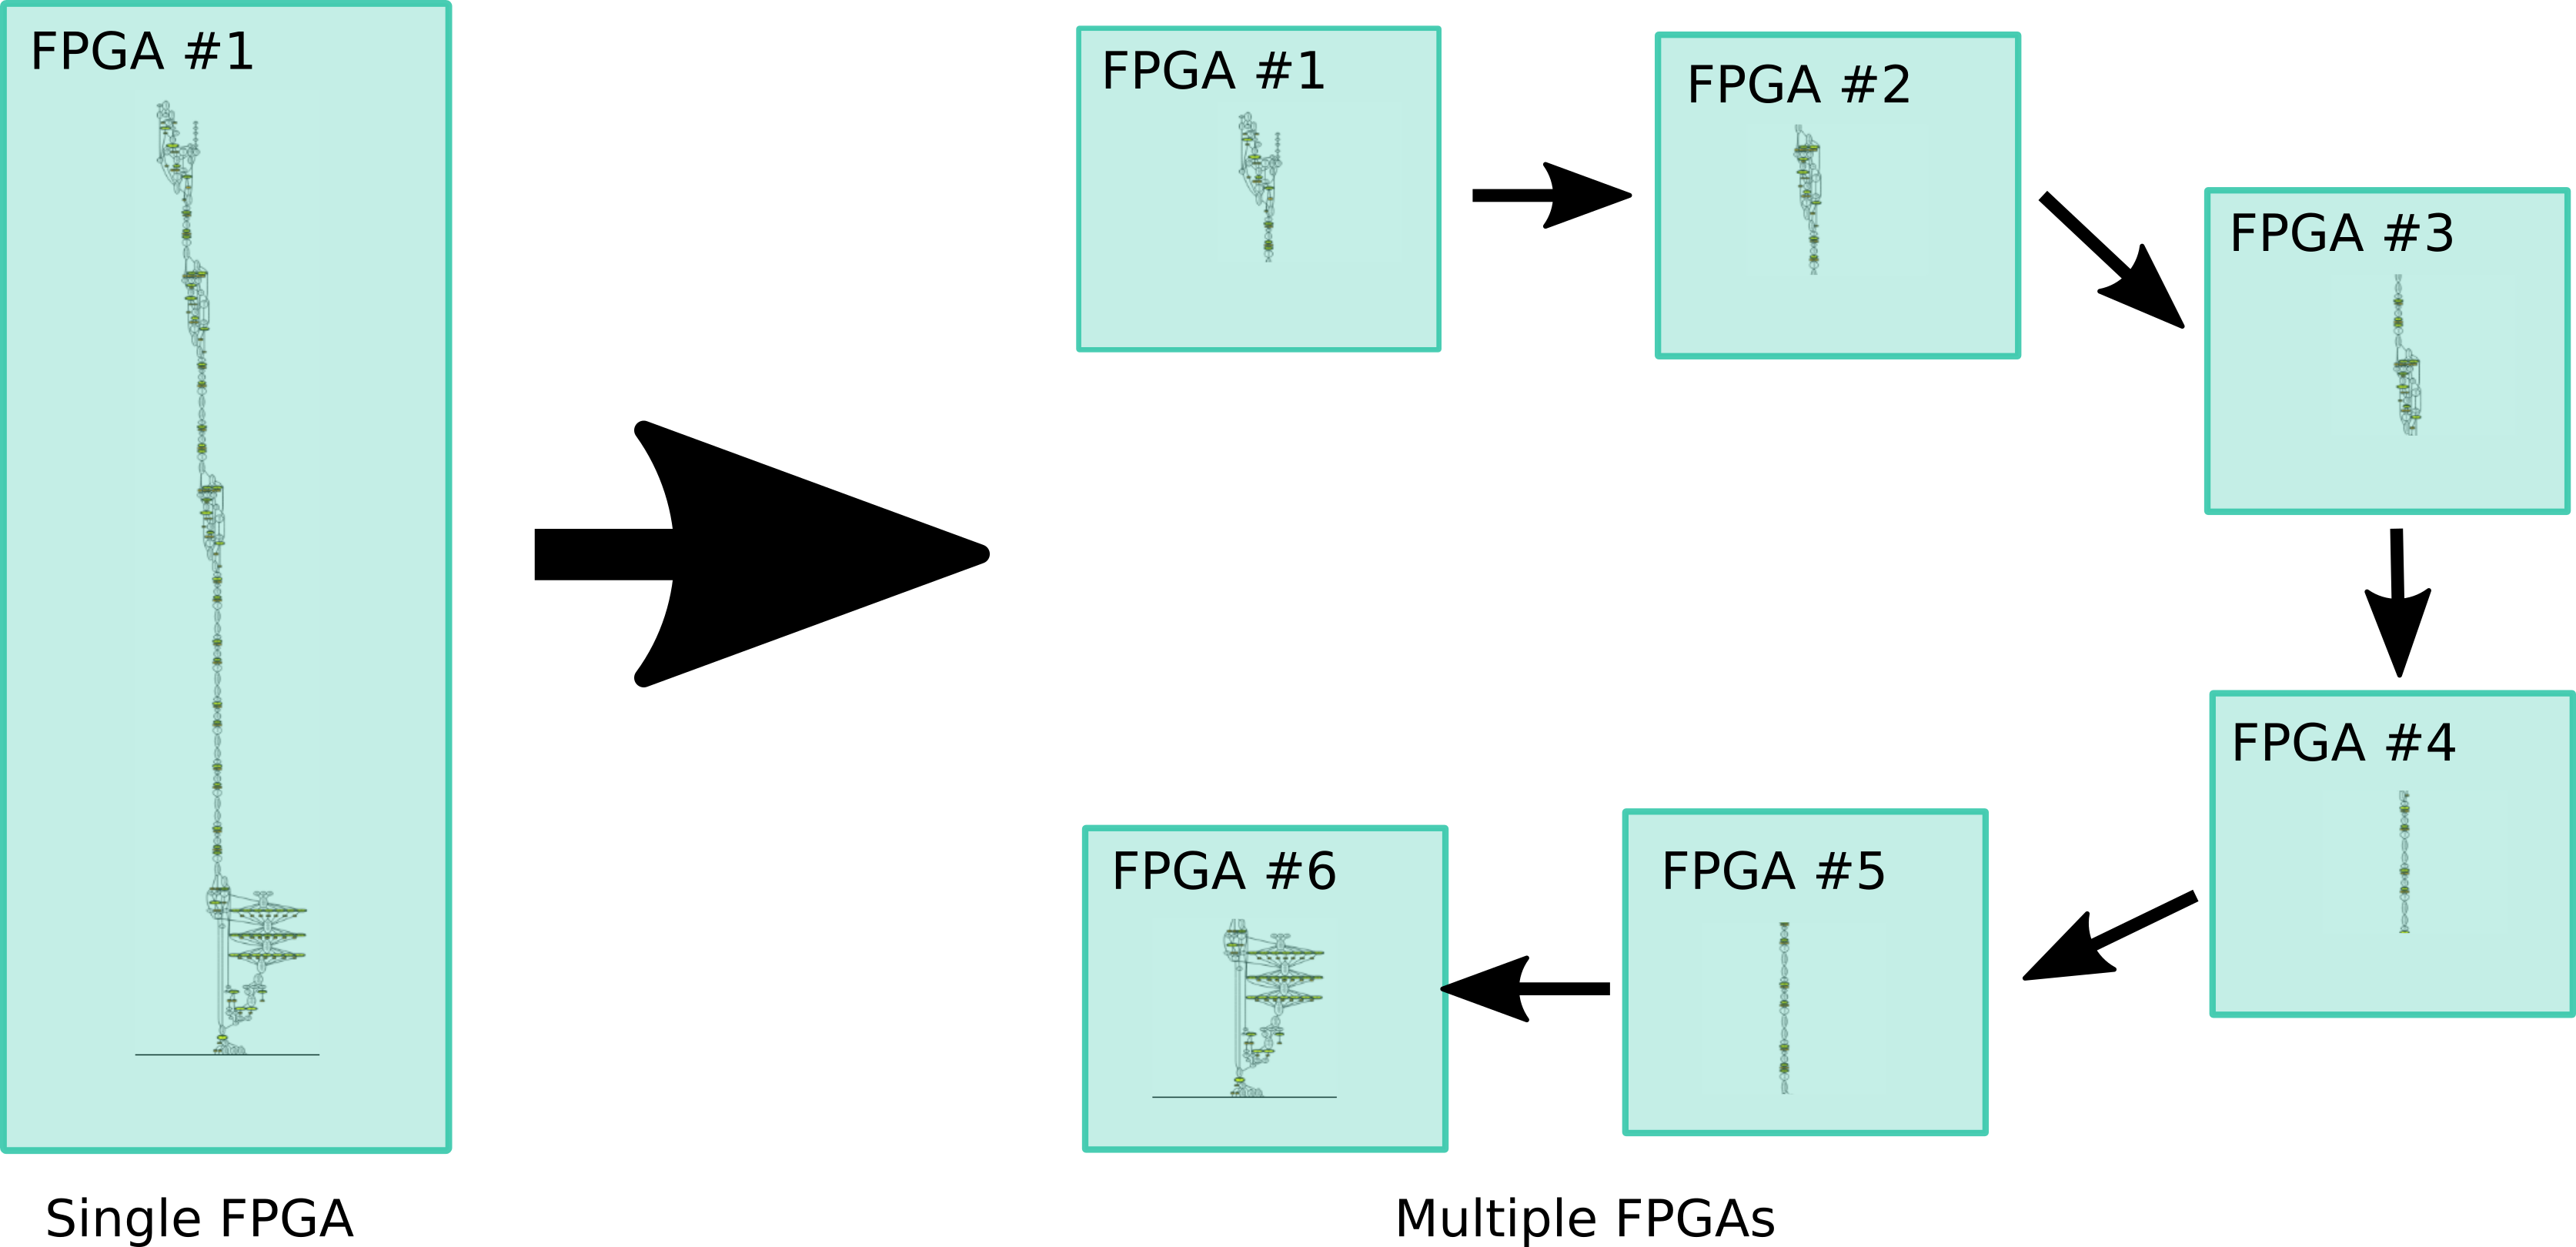
\includegraphics[width=1.0\textwidth]{drawings/dycore-estimate-split-design-multi-fpga.png}
	\caption{Split the problem into equal sized subproblems which fit on instanced of the re-programmable device. Stream the required data fields between them.}
	\label{fig:dycore-estimate-split-design-multi-fpga}
\end{figure}
